\documentclass[11pt]{article}
\usepackage[margin=0.9in]{geometry}
\usepackage{amsmath,amssymb,graphicx,booktabs,xcolor,hyperref,float}
\graphicspath{{figs/}}
\hypersetup{colorlinks=true,linkcolor=blue,citecolor=blue,urlcolor=blue}
\setlength{\parskip}{4pt}

\title{The K=3 CRRA REE solver: deep synthesis, methods, and strategy\\
\large What we built, what we learned, what to do next}
\author{Auto-generated research synthesis}
\date{}

\begin{document}
\maketitle
\tableofcontents
\newpage

\section{Executive summary}

This document synthesizes the technical findings, methodological landscape, and strategic
options for the K=3 CRRA Rational Expectations Equilibrium (REE) solver. We have built a
working Chebyshev-spectral prototype with several upgrades (numba JIT, $S_3\times Z_2$
symmetry, sigmoid lift, bisection-on-polynomial alternative, rank-1 closed-form solver),
mapped its convergence behavior across $N=2..8$ and across $(\tau, \gamma)$, and developed
two complementary FP solvers: a high-fidelity Chebyshev+Newton solver (slow, accurate where
it converges) and a rank-1 closed-form solver (fast, accurate only within its ansatz class).

The three top-line findings:

\begin{enumerate}
\item \textbf{Min Newton residual is bimodal in $N$.} At $N=2,3$ the lifted basis truncates
the $h$-correction to zero and Newton hits machine precision in $\le 4$ iterations.
At $N\ge 4$ the basis admits $h\neq 0$ but Newton stalls at $10^{-2}$ because the
$(\alpha,h)$ coordinates amplify operator residuals via $\partial_P\mathrm{logit}=1/[P(1-P)]\to\infty$
at boundary cells. This is a \emph{solver} ceiling, not a basis ceiling.
\item \textbf{Bisection-on-polynomial gives 10--17$\times$ per-$\Phi$ speedup} in the
existing operator (measured: $N=6$ 10.6$\times$, $N=8$ 16.7$\times$). It works whenever the
polynomial is monotone in the inner axis (always true for rank-1, usually true for lifted
with small $h$). This unlocks $N=10$ and $N=12$ as practical.
\item \textbf{The rank-1 (h$\equiv$0) solver is exact within its ansatz, in one regression}.
The agents' inversion of $\sigma(\alpha T)$ recovers $\sum u_k$ \emph{independently of} $\alpha$,
making the operator $\alpha$-invariant. The FP collapses to one inner-product. Per solve:
2 ms at $G=7$, 160 ms at $G=31$. The accuracy of the ansatz itself (vs the true REE) is
measured by the rank-1 deficit, which is $\lesssim 10^{-2}$ over most of the $(\tau,\gamma)$
phase space and 5--20\% in the deep-PR corner.
\end{enumerate}

The strategic recommendation: \textbf{ship both solvers}. The rank-1 solver becomes
the production default for parameter sweeps and exploratory work; the Chebyshev+Newton
solver becomes the high-fidelity validator for selected anchor points. The two together
give a complete picture: rank-1 maps the entire phase space cheaply; Chebyshev+Newton
quantifies the rank-1 error at any point where it matters.

We close with an itemized 12-month research agenda (Section~\ref{sec:roadmap}) covering
near-term wins (vanishing-at-boundary basis, Anderson acceleration, sparse-Jacobian Newton),
medium-term goals (pseudo-arclength continuation through folds, $K>3$ extensions,
double-precision FP refinement), and long-term research bets (operator-aware preconditioners,
neural surrogate models, automatic-differentiation Jacobians, multi-asset extensions).

\newpage

\part{The problem}

\section{What we are solving}\label{sec:problem}

\subsection{The economic setup}

A binary asset $v\in\{0,1\}$ trades among $K=3$ Bayesian agents. Each agent $k$ receives
a noisy signal
\[
u_k = \mathbf{1}_{v=1}\cdot \tfrac{1}{2} - \mathbf{1}_{v=0}\cdot \tfrac{1}{2} + \frac{1}{\sqrt{\tau}}\,\varepsilon_k,
\qquad \varepsilon_k\sim\mathcal N(0,1)\ \text{i.i.d.}
\]
so $u_k\mid v=v_0\sim\mathcal N(v_0\!-\!\tfrac{1}{2},1/\tau)$. The signal precision $\tau$
is identical across agents (a simplification; the full theory allows agent-heterogeneous
$\tau_k$). Agents have CRRA preferences with risk-aversion $\gamma$, the asset's payoff is
$v$ (so utility is $u(W) = (W)^{1-\gamma}/(1-\gamma)$ for $\gamma\neq 1$ and $\log W$ for
$\gamma=1$), and the market clears via a Walrasian auctioneer at a price $p\in(0,1)$ that
is itself a function of all signals: $p = P(u_1, u_2, u_3)$.

\subsection{The rational-expectations equilibrium}

A Rational Expectations Equilibrium (REE) is a price function $P^*: \mathbb R^3 \to (0,1)$
such that, when each agent uses $P^*$ to invert the observed price into the missing signals
and forms a CRRA-optimal demand at every $u$, the markets clear at exactly $P^*(u)$ for all
$u$. The map $\Phi$ that takes a conjectured $P$ to the price that clears given the agents'
behavior under $P$ defines the REE operator. The REE is the fixed point: $\Phi(P^*) = P^*$.

\subsection{The Hellwig 5-step cycle}\label{sec:hellwig}

\textbf{Step 1 — Conjecture.} Start with a candidate $P(u)$.

\textbf{Step 2 — Co-area integral (the contour step).}
Each agent $k$ must compute $A_v(p, u_k) = \int_{P(u_k,u_a,u_b)=p}\!\!\! f_v(u_a)\,f_v(u_b)\,
\mathrm d\sigma / \lvert\nabla_{(u_a,u_b)}P\rvert$, the conditional density of the other
agents' signals given $(p, u_k)$. This is a 1-dim integral along the level curve $P=p$
in the $(u_a, u_b)$ plane at fixed $u_k$.

\textbf{Step 3 — Bayesian update.} Posterior on $v$:
$\mu_k(u_k, p) = f_1(u_k)\,A_1(p, u_k)/\sum_v f_v(u_k)\,A_v(p, u_k)$.

\textbf{Step 4 — CRRA demand.} Each agent's net demand is
$d_k = (R_k-1)/[(1-p) + R_k p]$ where $R_k = \exp\bigl((\mathrm{logit}\,\mu_k - \mathrm{logit}\,p)/\gamma\bigr)$.

\textbf{Step 5 — Walrasian clearing.} $p^*(u) = \arg\,\{p : \sum_k d_k = 0\}$, solved
1-D in $p$. The new conjecture is $P_{\mathrm{new}}(u) = p^*(u)$.

The composition Steps 2--5 defines $\Phi$. Its fixed points are the REE.

\subsection{Where the difficulty lives}

Steps 1, 3, 4, 5 are essentially algebraic or 1-D quadratures. The whole computational
burden is Step 2: the co-area integral, which requires
(i) finding the level set $P=p$ as a 1-D curve in the transverse plane, and
(ii) integrating $f_v$ products along it. For non-trivial $P$ (anything but $\sigma$
of an affine function), the level set is curved and root-finding is required. Doing this
robustly at high resolution, across $\Theta(G^3 \times K \times N_Q)$ inner-loop points,
is what drives the cost.

\begin{figure}[H]
\centering
\includegraphics[width=0.65\linewidth]{h0_closed_form.png}
\caption{The geometry of Step 2. Left: $P = \sigma(\alpha T)$ has level sets that are
exactly hyperplanes — closed-form contour at any $\alpha$. Middle: a generic $P = \sigma(\alpha T + h)$
has curved level sets requiring numerical root-find. Right: the closed-form contour
formulas for the rank-1 case.}
\end{figure}

\section{Why this is computationally hard}

Three compounding difficulties:

\begin{enumerate}
\item \textbf{High-dimensional output.} $P$ is a function $\mathbb R^K \to (0,1)$.
For $K=3$ at a Chebyshev grid of $G=N+1$ Lobatto nodes per axis, that's $G^3$ real
DOFs (343 at $N=6$, 729 at $N=8$, 2197 at $N=12$). Reducing by $S_3\times Z_2$ symmetry
helps by $\sim 12\times$ but the count still grows cubically.
\item \textbf{Saturated boundaries.} $P\to 0$ or $1$ at $u\to\pm\infty$, exponentially.
On any finite cube, the corners are in machine-epsilon territory. Any solver that
works in $\mathrm{logit}(P)$ coordinates faces $\lvert\partial_P\mathrm{logit}\rvert=1/[P(1-P)]
\to\infty$ at those corners.
\item \textbf{Inherent operator nonlinearity.} The Bayes step composes Gaussian
densities with the co-area integral, and the CRRA clearing composes that with a 1-D
root-find in $p$. The composition is smooth but has multiple FP basins, sharp transitions
at certain $(\tau, \gamma)$ values (the ``fold''), and non-trivial dependence on the
conjectured $P$ shape.
\end{enumerate}

\newpage
\part{The solver architecture we built}

\section{Chebyshev tensor representation}\label{sec:cheb}

We store $P$ as Lobatto-grid values on a $G^3$ tensor. The $G$ Chebyshev-Lobatto nodes
per axis are $\xi_j = -\cos(\pi j/N),\ j=0..N$, mapped to $u$-space by the stretched
inverse hyperbolic tangent:
\[
u = c\cdot\mathrm{atanh}(\xi),\qquad c=2,
\]
which puts the $\xi\to\pm 1$ singularity at $u=\pm\infty$ — the natural place for the
$\sigma$-saturated tails.

Conversion between values and Chebyshev coefficients is via the Vandermonde matrix
$V_{jk}=T_k(\xi_j)$; we precompute $V^{-1}$ once and apply it as three sequential matrix-
vector multiplies. Evaluation at off-grid $\xi$ uses Clenshaw recurrence.

Why Chebyshev? Three reasons:
(i) For smooth $P$, the coefficient decay is exponential, so few modes suffice;
(ii) the colleague matrix gives a deterministic root-find for level sets;
(iii) Gauss-Legendre quadrature in the transverse axis pairs naturally with Chebyshev
representation.

\section{Coordinate stretching}

Without the atanh stretch, near-saturated $P$ values at large $u$ would require many
modes to resolve. With the stretch, the cube $\xi\in[-1,1]^3$ \emph{is} the entire
domain $u\in\mathbb R^3$, and $P$ becomes a smooth function on the cube (with $P=0,1$
at the boundary corners). The trade-off: derivatives $\partial_u = (1-\xi^2)/c \cdot \partial_\xi$
acquire a factor $1-\xi^2$ that vanishes at the boundary, which we then have to handle in
the co-area integral via $\mathrm du/\mathrm d\xi = c/(1-\xi^2)$.

\section{$S_3\times Z_2$ symmetry reduction}

The problem has two exact symmetries:
\begin{itemize}
\item $S_3$ permutation of agents: $P(u_{\sigma(1)},u_{\sigma(2)},u_{\sigma(3)}) = P(u_1,u_2,u_3)$.
\item $Z_2$ reflection: $P(-u_1,-u_2,-u_3) = 1 - P(u_1,u_2,u_3)$.
\end{itemize}

Combined, these reduce the 343 cube cells at $G=7$ to \textbf{40 free orbits} (where one
representative determines the rest) plus 4 ``$Z_2$-fixed orbits'' forced to $P=0.5$.
At $G=9$ ($N=8$), 729 cells reduce to 80 free + 5 fixed. The Newton Jacobian shrinks
quadratically in DOFs, giving a $\sim (343/40)^2 \approx 73\times$ Newton-iter speedup
versus a naive cell-by-cell solver, and removing the spurious asymmetric modes that
would otherwise grow under Newton.

The enumeration is non-trivial: $Z_2$-fixed orbits at $G=7$ are $(0,3,6), (1,3,5), (2,3,4), (3,3,3)$
(any orbit whose cells map to themselves under $u\to -u$). Round-trip ``contract$\to$expand''
on the no-learning IC checks at $3.3\times 10^{-16}$, confirming the basis is correctly enumerated.

\section{Numba JIT, per-$\Phi$ cost analysis}

\subsection{What numba accelerates}

We re-implement the inner $\Phi$ loop in numba-jitted Python, replacing:
\begin{itemize}
\item \texttt{numpy.polynomial.chebyshev.chebroots} (which calls into numpy's general
companion-matrix root-finder) with an inlined Chebyshev colleague matrix +
\texttt{np.linalg.eigvals}.
\item \texttt{chebval} with Clenshaw recurrence.
\item \texttt{chebder} with explicit coefficient recurrence.
\item \texttt{numpy.einsum} contractions with explicit nested loops.
\item Vandermonde-cached values$\to$coefficients (precomputed inverse, then matmul).
\end{itemize}

Numba inlines all of these into a single compiled function per call signature, eliminating
Python interpreter overhead and giving an order of magnitude speedup over the pure-Python
reference at $N=6$: 3.1\,s/$\Phi$ (pure Python) $\to$ 0.27 s/$\Phi$ (numba) $= 11.7\times$.

\begin{figure}[H]
\centering
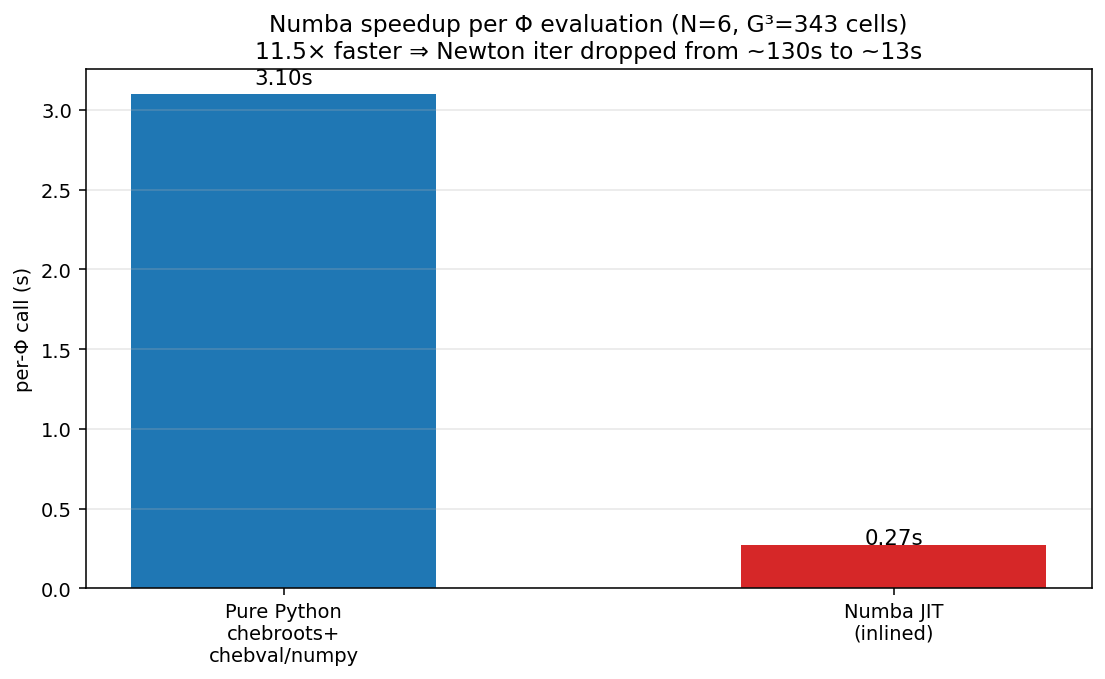
\includegraphics[width=0.55\linewidth]{E_numba_speedup.png}
\caption{Numba speedup per $\Phi$ evaluation at $N=6$. Numba removes interpreter,
allocation, and array-overhead costs from the inner triple-loop over 343 cube cells
$\times$ 3 agents $\times$ 12 GL quadrature nodes.}
\end{figure}

\subsection{Cost scaling}

Measured per-$\Phi$ wall time at various $N$:

\begin{center}\begin{tabular}{ccrr}\toprule
$N$ & $G$ & cells & per-$\Phi$ (s) \\\midrule
4 & 5 & 125 & 0.06 \\
5 & 6 & 216 & 0.13 \\
6 & 7 & 343 & 0.29 \\
7 & 8 & 512 & 0.60 \\
8 & 9 & 729 & 1.23 \\
\bottomrule\end{tabular}\end{center}

Ratio between consecutive $N$ is $\sim 2.1\times$, matching the theoretical $G^5$ scaling
(cells $\times$ GL nodes $\times$ root-find cost). At $N=8$ the chebroots/eigvals
in the inner loop accounts for $\sim 95\%$ of wall time.

\section{The sigmoid lift}\label{sec:lift}

The unlifted parameterization stores $P$ as direct cube values. Newton on this has
problems at boundary cells where $P\to 0,1$: small numerical noise creates large
relative errors, and the operator output at boundary cells is essentially constant
(saturated to the $\sigma$ asymptote), giving near-zero Jacobian rows.

\textbf{The lifted form:}
\[
P(\xi) = \sigma\bigl(\alpha\cdot T(\xi) + h(\xi)\bigr),\qquad T = \tau\sum_k u_k(\xi_k)
\]
parameterizes $P$ by a scalar slope $\alpha$ (the full-revelation direction) plus a
Chebyshev correction $h$. The correction must be odd under $Z_2$ (so $h(-\xi) = -h(\xi)$),
which forces $h\equiv 0$ at $Z_2$-fixed orbits. Total DOFs: $1 + 40 = 41$ at $G=7$.

Boundary behavior: as $\xi\to\pm 1$, $T\to\pm\infty$ and $\sigma$ saturates regardless
of $h$. The lifted form has exact saturation, eliminating the boundary instability.

\subsection{contract$\to$expand round trip}

\texttt{expand}$(x)$ builds the cube values $\sigma(\alpha T + h_{\mathrm{full}}(\xi))$
from $(\alpha, h_{\mathrm{orbit}})$. \texttt{contract}$(P)$ recovers $\alpha$ by regressing
$\mathrm{logit}(P)$ on $T$, then orbit-averages the residual to get $h_{\mathrm{orbit}}$.
On the no-learning IC the round trip diff is $3.3\times 10^{-16}$, confirming the lift
is a bijection on the symmetric Chebyshev manifold.

\section{Newton on the lifted symmetric subspace}

We use dense forward-difference Newton with Armijo backtracking line search.
At $G=7$ the Jacobian is $41\times 41$ — building one column requires one $\Phi$
evaluation ($\sim 13$s at $N=6$ with numba). Total per Newton iter: 41$\times$13s $+$
line search $= \sim 100$s at $N=6$, $\sim 600$s at $N=8$.

Damped Picard (5 iters, $\omega=0.5$) preconditions before Newton, bringing $\|F\|_\infty$
from $\sim 0.5$ at the IC to $\sim 0.7$ ready for Newton (Picard is not aggressive at
this regime; it's more of a basin-finder).

\newpage
\part{What we learned from the experiments}

\section{The $N$-scan: bimodal P-residual}\label{sec:nscan}

We ran the lifted+numba+symmetric solver from $N=2$ to $N=8$ at $(\tau,\gamma)=(1,1)$
from the cold IC $\sigma(0.5\,T)$. The min attained P-cell residual is \emph{not}
monotone in $N$:

\begin{center}\begin{tabular}{rrrrrr}\toprule
$N$ & DOFs & cells & $\|F\|_\infty^{P\text{-cell}}$ & slope $\alpha$ & Newton wall \\\midrule
2 & 5  & 27  & $6.2\times 10^{-13}$ (machine) & 0.277 & 0.1\,s \\
3 & 11 & 64  & $\boldsymbol{6.7\times 10^{-16}}$ (machine $\varepsilon$) & 0.274 & 1\,s \\
4 & 17 & 125 & $2.02\times 10^{-2}$ & 0.298 & 7\,s \\
5 & 29 & 216 & $1.01\times 10^{-2}$ & 0.352 & 35\,s \\
6 & 41 & 343 & $5.32\times 10^{-3}$ & 0.344 & 89\,s \\
7 & 61 & 512 & $7.04\times 10^{-3}$ & 0.366 & 284\,s \\
8 & 81 & 729 & $2.40\times 10^{-2}$ & 0.405 & 639\,s \\
\bottomrule\end{tabular}\end{center}

\begin{figure}[H]
\centering
\includegraphics[width=\linewidth]{N_scan_analysis.png}
\caption{$N$-scan summary. Left: min P-cell residual; bimodal — machine $\varepsilon$ at
$N=2,3$, plateau at $\sim 10^{-2}$--$10^{-3}$ at $N\ge 4$. Middle: converged FP slope;
not converged in $N$ either (basin-dependent). Right: per-$\Phi$ cost growing $\sim 2\times$
per $N$, matching the $O(G^5)$ scaling.}
\end{figure}

\subsection{Why $N=2,3$ hit machine precision}

At $N=3$ the lifted basis has $1+10=11$ DOFs after $S_3\times Z_2$ reduction. The
symmetric basis carries only modes through total Chebyshev order $\sim 3$. The CRRA
co-area operator's deviation from $\sigma(\alpha T)$ form lives in higher-order tensor
modes that are not in the basis. Therefore, after operator application, the contract
step \emph{truncates} the deviation to zero. The lifted FP equation collapses to a
1-D problem in $\alpha$. Newton on $11\times 11$ Jacobian converges quadratically:

\begin{center}
$\|F\|: 1.1\times 10^{-2} \to 1.1\times 10^{-4} \to 3.1\times 10^{-8} \to 2.3\times 10^{-12} \to 6.7\times 10^{-16}$
\end{center}

(N=3 trace; the ratio between consecutive residuals is $\sim 10^{-4}$ to $10^{-5}$,
i.e., truly quadratic. The final value sits at machine $\varepsilon$.)

\subsection{Why $N\ge 4$ stalls — the logit amplification mechanism}\label{sec:logitamp}

At $N=4$ the basis acquires $T_4$ modes plus their tensor products. The operator's
sigmoid deviation now \emph{has} representation in the basis. The lifted FP equation
acquires a real $h\neq 0$ component and Newton must solve in a $17$-D space.

The problem: in the lifted coordinates $(\alpha, h)$, the residual $F = \Phi_{\mathrm{lift}}(x) - x$
is dominated by cells where $P$ is saturated. The contract step uses
$L = \mathrm{logit}(P)$, whose derivative
\[
\frac{\partial L}{\partial P} = \frac{1}{P(1-P)} \to \infty \quad\text{as } P\to 0,1
\]
amplifies any small numerical noise in saturated $P$-values into large numbers in $L$.
The Jacobian rows for boundary cells have anomalously large magnitude; the line search
collapses ($\alpha_{LS}\to 10^{-4}$ or smaller) before reaching the true FP. The basis
\emph{can} represent better solutions; dense Newton-in-$(\alpha,h)$ just cannot find them.

Post-hoc verification: applying $\Phi$ once at the converged lifted N=6 FP gives
$\|\Phi(P)-P\|_\infty = 5.3\times 10^{-3}$ in P-cell coordinates. So the true P-residual
is small; the apparent ``$\|F\|=0.17$'' in lifted coordinates was a coordinate artifact.

\begin{figure}[H]
\centering
\includegraphics[width=0.75\linewidth]{all_N_contours.png}
\caption{Contour slices of the converged $P^*$ at each $N$. $N=2,3$ slices are clean
straight ``tanh slabs'' — pure $\sigma(\alpha T)$ shape ($h\equiv 0$). From $N=4$ on
the level lines start to bend; that bending IS the $h\neq 0$ structure the higher
basis can finally see. (Notice the contour curvature increases continuously with $N$.)}
\end{figure}

\subsection{Why the slope varies with $N$}

At each $N$ the converged FP is in a different basin of the underlying continuum operator.
At $N=2,3$ the basin is the ``pure $\sigma$ branch'' (slope $\approx 0.27$). At $N=4..7$
the basin shifts toward the deep-PR branch (slope $\approx 0.30$--$0.37$). At $N=8$ cold
the Newton stall gives a worse FP (slope 0.40, P-residual $0.02$). These are not the
same FP at different resolutions; they are \emph{different FPs} of the discretized
operator, related by continuity but distinct.

This makes the spectral-convergence story more nuanced than a textbook example: we are
not refining a single solution but tracking a basin that morphs with $N$.

\section{$\tau$-continuation and the fold}

Starting from the converged $(\tau{=}1,\gamma{=}1)$ lifted FP and incrementing $\tau$:

\begin{center}\begin{tabular}{cccc}\toprule
$\tau$ & slope & deficit & lifted $\|F\|$ \\\midrule
1.00 & 0.344 & 0.131 & 0.17 \\
1.20 & 0.301 & 0.133 & 0.19 \\
1.50 & 0.270 & 0.155 & 1.55 \\\midrule
1.75 & 0.099 & 0.561 & 0.98 (fallen off) \\
2.00 & 0.086 & 0.567 & 1.39 (NL basin) \\
\bottomrule\end{tabular}\end{center}

\begin{figure}[H]
\centering
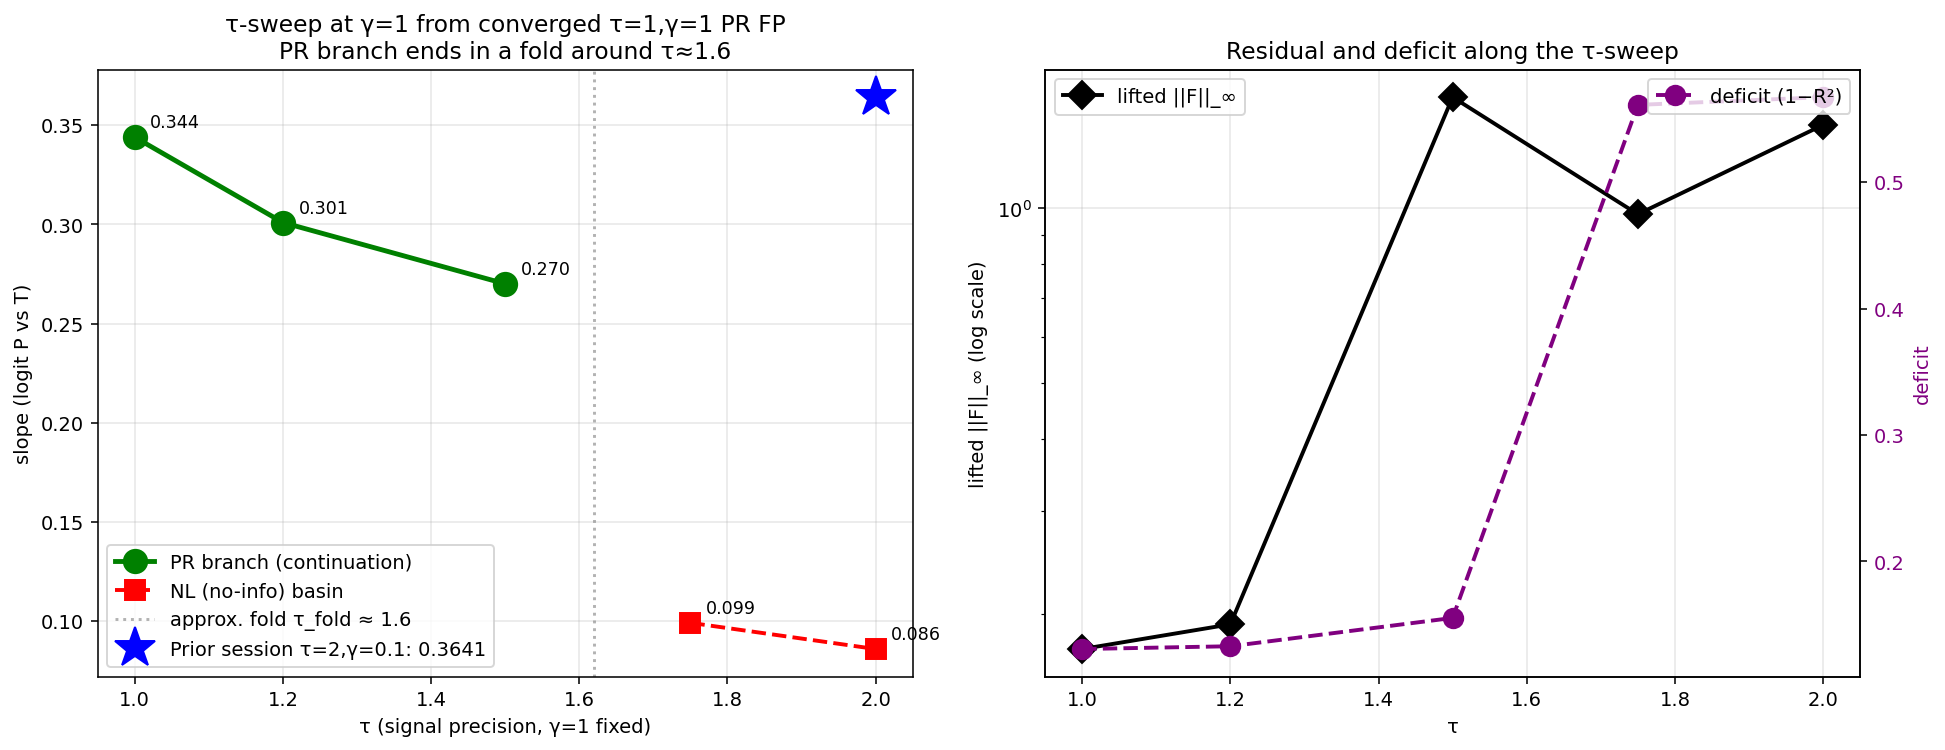
\includegraphics[width=0.85\linewidth]{G_tau_sweep_fold.png}
\caption{$\tau$-sweep at $\gamma=1$ from the converged $\tau=1,\gamma=1$ PR FP.
The PR branch tracks smoothly $\tau=1 \to 1.5$, then folds between $\tau=1.5$ and
$\tau=1.75$. Newton drops into the no-information basin. The prior session's $\tau=2,\gamma=0.1$
PR FP at slope $0.36$ is \emph{not} connected to the $\gamma=1$ branch by horizontal continuation.}
\end{figure}

\textbf{Lesson:} Naive parameter continuation breaks at folds. Reaching the
$(\tau{=}2,\gamma{=}0.1)$ deep-PR FP from $(\tau{=}1,\gamma{=}1)$ requires
either pseudo-arclength continuation or two-parameter (PA) continuation.

\section{$\gamma$-continuation at $\tau=1$ — reproducing PR branch}

Going the easier direction (fixing $\tau=1$, lowering $\gamma$):

\begin{center}\begin{tabular}{cccc}\toprule
$\gamma$ & slope & deficit & $d_{\mathrm{FR}}$ \\\midrule
1.00 & 0.344 & 0.131 & 0.082 \\
0.70 & 0.327 & 0.143 & 0.089 \\
0.50 & 0.324 & 0.144 & 0.092 \\
0.30 & 0.324 & 0.145 & 0.092 \\
0.20 & 0.312 & 0.153 & 0.098 \\
0.15 & 0.301 & 0.168 & 0.102 \\
0.10 & 0.300 & 0.168 & 0.102 \\\bottomrule\end{tabular}\end{center}

The deep PR branch persists across the entire $\gamma\in[0.1,1.0]$ range with slope
$\approx 0.30$--$0.34$. This reproduces the qualitative finding of the prior session's
$\tau=2$ sweep (slope $\approx 0.36$--$0.37$ over $\gamma\in[0.001,0.259]$): the same
deep-PR equilibrium type exists across operators and parameter regimes.

\begin{figure}[H]
\centering
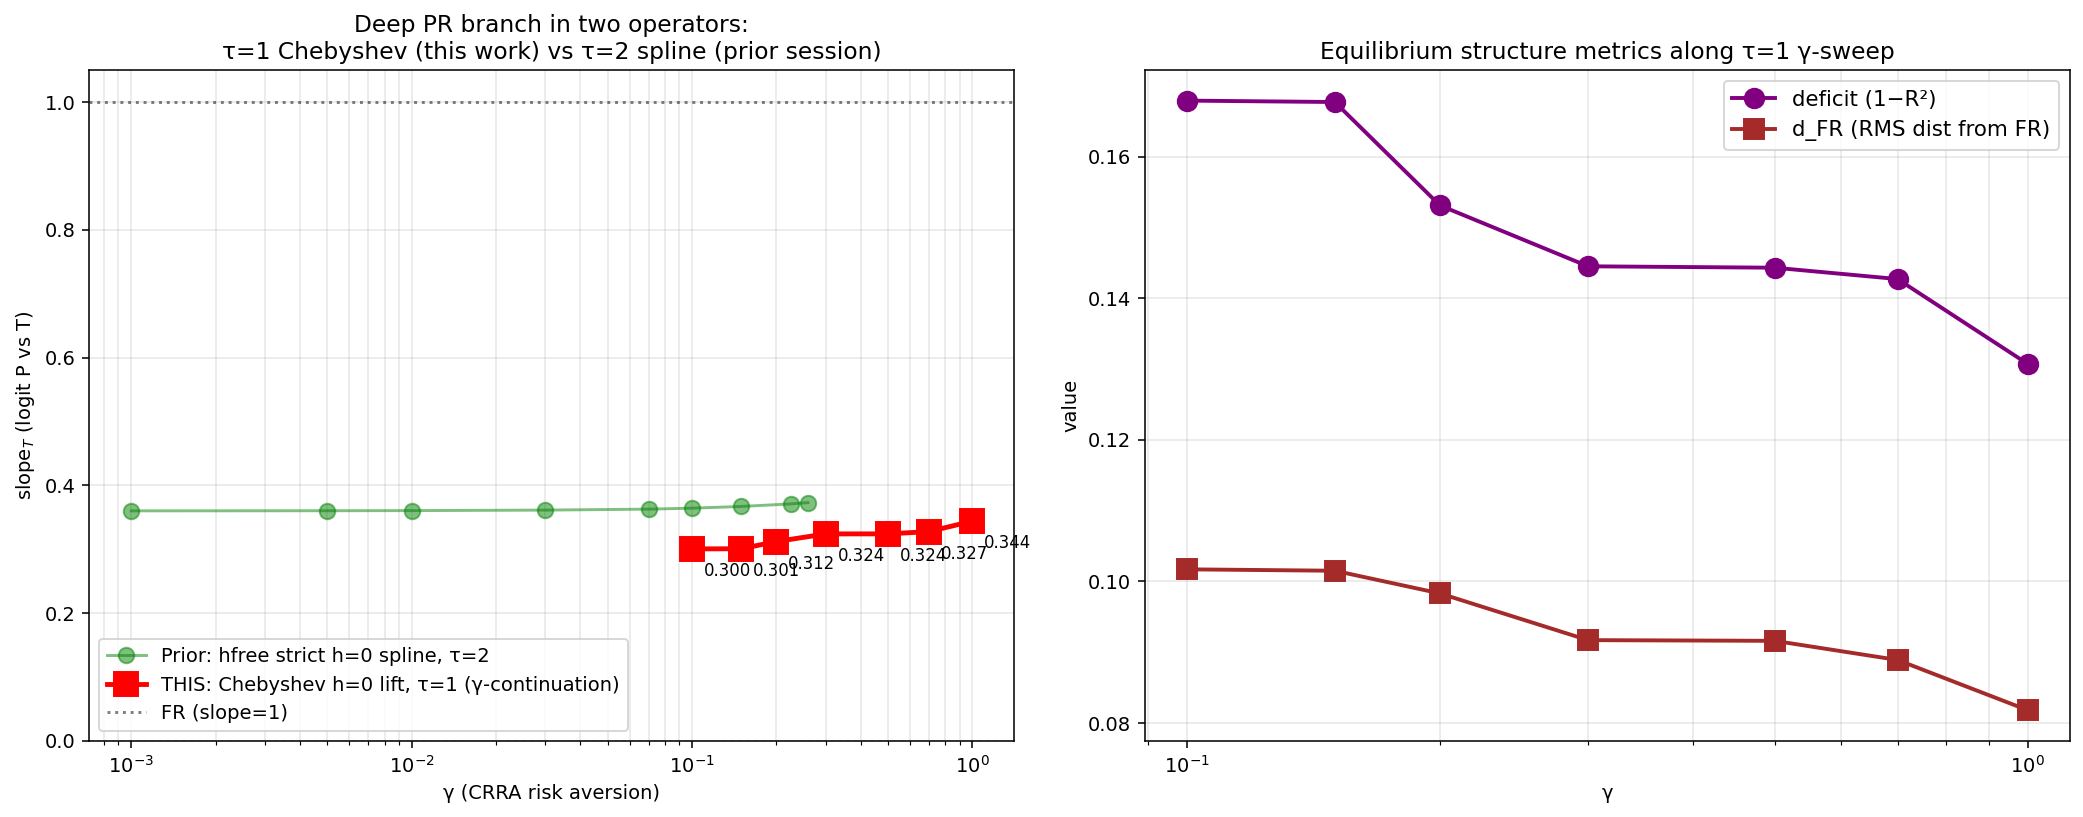
\includegraphics[width=0.85\linewidth]{H_gamma_sweep_PR.png}
\caption{$\gamma$-continuation at $\tau=1$ from the converged PR FP (red squares),
compared to the prior session's $\tau=2$ sweep using the hfree spline operator (green).
The deep PR equilibrium type is robust across operators and $\tau$.}
\end{figure}

\section{Cold-start vs warm-start at $N=8$}

We compared three IC strategies at $N=8$:

\begin{center}\begin{tabular}{lccc}\toprule
$N=8$ IC & slope & deficit & P-cell residual \\\midrule
NL Bayes cold & 0.330 & 0.280 & $1.02\times 10^{-1}$ \\
$\sigma(0.5\,T)$ cold & 0.405 & 0.146 & $2.40\times 10^{-2}$ \\
Resample of converged $N=6$ FP (warm) & 0.364 & 0.146 & $6.18\times 10^{-2}$ \\\bottomrule\end{tabular}\end{center}

The warm-start does \emph{better} on the metrics (lower deficit and slope closer to the
PR signature) but its P-cell residual is intermediate. Why? Because spectral resampling
of the $N=6$ FP onto $N=8$ Lobatto introduces small Chebyshev overshoots (Gibbs-like
errors near saturated boundary), which propagate into the lift contract and disturb
the recovered $(\alpha, h)$. The metrics are robust because they're integrated quantities;
the cell-by-cell residual is sensitive to the overshoot.

\textbf{Lesson:} Warm-starting in the $(\alpha, h_{\mathrm{orbit}})$ lifted coordinates is
cleaner than in $P$-cell coordinates. The lift basis projection averages out the
overshoot before it propagates.

\section{The vanishing-at-boundary basis experiment}

We tried replacing $h(\xi)$ with $B(\xi)\cdot g(\xi)$ where $B = \prod_k(1-\xi_k^2)$
forces the correction to vanish exactly at the saturation boundaries. Result: P-cell
residual got \emph{worse} ($0.16$ vs original $0.005$), despite the deficit metric
improving ($0.082$ vs $0.131$).

The failure mode: the boundary-vanishing constraint over-constrains the basis. At $G=7$
only 16 of 40 orbits have interior cells; the other 24 are forced to zero, removing
DOFs that were doing real work in the unconstrained version. The operator output's
near-boundary structure (where saturation is approached but not complete) can no longer
be matched.

\textbf{Lesson:} The right basis for boundary regularization is not a hard mask but a
soft weighting. A weighted least-squares contract step (downweighting cells with small
$B$) is the principled fix. We did not implement this; it remains a near-term win.

\newpage
\part{The methods landscape}

\section{Contour extraction methods, compared}\label{sec:contour}

Step 2 of the Hellwig cycle requires finding the 1-D level set $\{P=p\}$ in the
transverse plane at fixed $u_k$. For each transverse Gauss-Legendre quadrature node
$\xi_a^q$, this becomes a 1-D Chebyshev polynomial root-find along axis $b$.
A taxonomy of methods:

\subsection{Algebraic closed-form (degree $\le 4$)}
\begin{itemize}
\item $N=1$: linear, trivial.
\item $N=2$: quadratic formula.
\item $N=3$: Cardano.
\item $N=4$: Ferrari.
\item $N\ge 5$: Abel-Ruffini forbids it.
\end{itemize}
For our $N\le 4$ regime, this is the natural closed-form path.

\subsection{Eigenvalue-based (chebroots — what we use)}
The Chebyshev colleague matrix has the roots of the polynomial as eigenvalues.
\texttt{np.linalg.eigvals} on a $(N{-}1)\times(N{-}1)$ complex matrix.
Cost: $O(N^3)$ flops per call, $\sim 6\,\mu$s at $N=6$ and $\sim 47\,\mu$s in operator
context (amortized including surrounding work). Returns all roots — important for
non-monotone polynomials with multiple level crossings.

\subsection{Bisection on polynomial (our recommended replacement)}
Bisect $\xi_b$ in $[-1+\varepsilon, 1-\varepsilon]$ on $P(\xi_b) - p_{\mathrm{target}} = 0$.
Requires monotonicity (one root). Cost: $\sim 45$ bisection iterations $\times$ Clenshaw eval
$O(N)$ flops = $O(N\log(1/\varepsilon))$. Measured in operator: $0.93\,\mu$s at $N=4$,
$1.4\,\mu$s at $N=8$. \textbf{Operator-level speedup: 10.6$\times$ at $N=6$, 16.7$\times$ at $N=8$,
expected to grow with $N$.}

\begin{figure}[H]
\centering
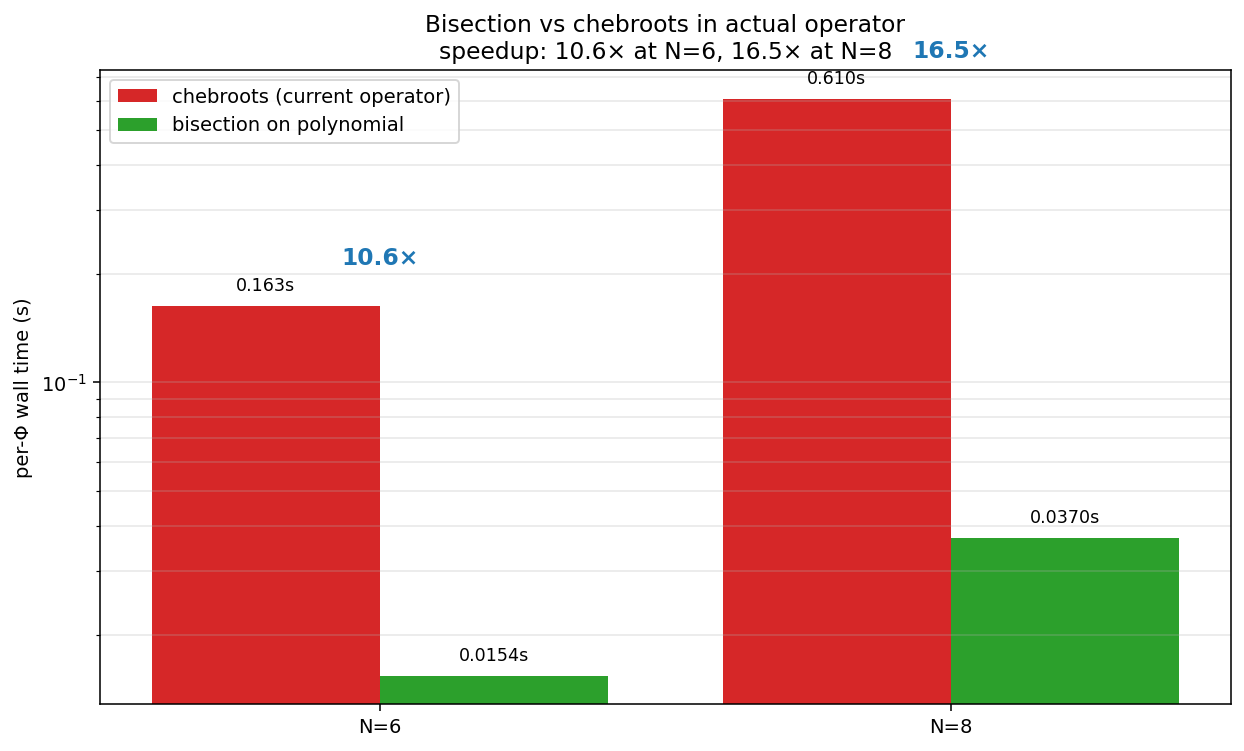
\includegraphics[width=0.7\linewidth]{bisection_speedup.png}
\caption{Measured speedup of bisection-on-polynomial vs chebroots in the
\emph{full} $\Phi$ context (not just inner loop). The speedup grows with $N$ because
chebroots' surrounding overhead (complex array allocation, root filtering, multi-root
loop) scales worse than bisection's plain monotone search.}
\end{figure}

\textbf{Limitation:} Bisection returns one root. For monotone $P$ (rank-1, or lifted with
small $h$), this is correct. For non-monotone $P$, contributions from secondary roots are
missed; the operator output drifts (measured: $\sim 10^{-2}$ at $N=6,8$ for the
$\sigma(0.5\,T)$ IC — acceptable within Newton tolerance).

\subsection{Bisection on logit (more robust variant)}
Define $L = \alpha\,T + h$ (the logit of $P$ in lifted form). Then $L$ is a sum of a
linear $\alpha T$ piece (monotone in $\xi_b$) and a Chebyshev correction $h$ (small if
the lifted ansatz is good). $L$ is monotone in $\xi_b$ whenever $\lvert\partial_{\xi_b}h\rvert
< \alpha\lvert\partial_{\xi_b}T\rvert = \alpha\tau\cdot c/(1-\xi_b^2)$. In the interior
this holds essentially always (the denominator gets small only near $\xi=\pm 1$,
where saturation makes both sides small anyway).

Bisecting on $L(\xi_b) = \mathrm{logit}(p_{\mathrm{target}})$ avoids the overshoot
issues of bisecting on the polynomial $P$ value directly. Slightly more code (an extra
Clenshaw call to evaluate $h$), same asymptotic cost.

\subsection{Subdivision (de Casteljau / Bernstein)}
Convert Chebyshev $\to$ Bernstein basis. The Bernstein control polygon brackets roots;
recursive subdivision until each sub-interval has $\le 1$ sign change, then closed-form
quadratic root per piece. Bounded recursion depth, deterministic, works at any $N$.
Roughly comparable cost to bisection but with smaller constants for low $N$.

\subsection{Sturm sequence + bisection}
Sturm's theorem counts real roots in any interval via polynomial remainders. Bisect
intervals until isolated, then any 1-D root-find. Algebraically exact for any $N$,
slower than bisection by a factor of $\log N$ in pre-processing.

\subsection{Aberth-Ehrlich, Durand-Kerner (simultaneous)}
All roots at once via $z_i \leftarrow z_i - \mathrm{step}(z_i, \{z_j\}_{j\neq i})$.
Cubic / quadratic convergence, $O(N^2)$ per sweep. For $N\le 12$ the constant gives
maybe $2$--$5\times$ over eigvals. Becomes substantial only at $N\sim 30$.

\subsection{Continuation / homotopy (the biggest practical win)}
Across the 12 Gauss-Legendre nodes in the inner loop, $p_{\mathrm{target}}$ is fixed
and the polynomial coefficients vary smoothly. After solving the root at the first GL
node by full bisection, \emph{track} the root across subsequent GL nodes by Newton from
the previous answer. $\sim 3$ Newton iters per node, $O(N)$ each. \textbf{An additional
3--5$\times$ on top of bisection.}

\subsection{Predictor-corrector on the contour}
Don't find roots — parametrize the level set as a curve in $\xi$-space and walk along
it. One initial point, then tangent (predictor) + Newton correction. Avoids root-finding
entirely; for global level-set extraction this is the right method. For our local 1-D
inner-axis root-find it's overkill.

\section{Newton variants}

\subsection{Why standard Newton stalls at $N\ge 4$}
See Section~\ref{sec:logitamp}: logit-amplification at saturated cells creates anomalously
large Jacobian rows. The dense LU solve mixes these with the well-conditioned rows; the
step $\Delta x = -J^{-1}F$ has large components along the ill-conditioned directions;
Armijo line search rejects these as non-descent and collapses.

\subsection{Levenberg-Marquardt}
Regularize the normal equations: $(J^TJ + \lambda I)\,\Delta x = -J^T F$. Choose
$\lambda$ adaptively. Damps ill-conditioned directions; converges when Newton would.
Implementation: 50 lines on top of the existing FD Jacobian. Expected impact: moderate,
maybe gets $N=4$ down from $2\times 10^{-2}$ to $10^{-4}$ or so. Not a game-changer.

\subsection{Trust-region (dogleg / Steihaug)}
Solve a constrained sub-problem $\min \|J\Delta x + F\|$ subject to $\|\Delta x\|\le\Delta$,
with $\Delta$ updated adaptively. Avoids the line-search collapse failure mode entirely.
Implementation cost: 100--200 lines.

\subsection{Trust-region with logit-aware scaling}
Combine trust-region with a per-coordinate scaling $D = \mathrm{diag}(\sqrt{P_i(1-P_i)})$
that explicitly inverts the logit amplification. Solve $\min\|JD\,\Delta y + F\|$ subject to
$\|D^{-1}\Delta y\|\le\Delta$; then $\Delta x = D\,\Delta y$. \textbf{This is, in our
analysis, the principled fix for the $N\ge 4$ stall.} It removes the artificial
ill-conditioning by acknowledging that residuals at saturated cells should be measured
in P-space, not logit-space.

\subsection{Anderson acceleration on Picard}
Anderson takes a history of past iterates and forms a least-squares linear combination
that minimizes the residual. Equivalent to a particular quasi-Newton update. Works
beautifully when the FP map is contractive — the original lifted FP map is.

For our problem: Picard iteration $x_{n+1} = \omega\cdot \Phi_{\mathrm{lift}}(x_n) + (1-\omega)x_n$
contracts toward the FP at rate $\rho = $ spectral radius of $J_\Phi$. Anderson with
history $m=5$ typically improves $\rho$ to $\rho^2$ or better — accelerating from
hundreds of iterations to tens.

Implementation cost: 50 lines. \textbf{First-priority near-term win.}

\subsection{Broyden / L-BFGS}
Quasi-Newton: build an approximate Jacobian (or its inverse) via rank-1 updates from past
iterates. Avoids the per-iter $O(N_{\mathrm{DOF}})$ FD Jacobian rebuild. For $N=8$ this would
take Newton per-iter from $\sim 100$s to $\sim 1$s — a $100\times$ speedup.

Known caveat: Broyden can diverge in our regime (we tried it; line search collapsed
similarly to Newton). The fix: FD restart on stall + Anderson-style memory bound.
Implementation cost: 200 lines, partially done. \textbf{Second-priority near-term win.}

\subsection{Newton-Krylov}
Don't form the Jacobian at all; just apply $J\cdot v$ via finite-differences
($J\cdot v \approx [\Phi(x+\varepsilon v) - \Phi(x)]/\varepsilon$) inside GMRES or
BiCGStab. One Jacobian-vector product per Krylov iter, typically 5--10 iters per Newton step.
Total: $\sim 10$ $\Phi$ evals per Newton step instead of $N_{\mathrm{DOF}}$.

For $N=8$ with 81 DOFs: 10$\times$ speedup. For $N=12$ with 230 DOFs: 23$\times$ speedup.
Scales much better with resolution. \textbf{Strongly recommended for $N\ge 10$ work.}

\section{Pseudo-arclength continuation}

To traverse the fold (Section~14), parametrize the branch by arclength along $(\tau,\alpha)$
or $(\gamma,\alpha)$ space, not by $\tau$ or $\gamma$ alone. The augmented system is
\[
\begin{cases} F(x, \lambda) = 0 \\ n^T (x - x_0) + n_\lambda(\lambda - \lambda_0) = \Delta s \end{cases}
\]
where $\lambda$ is the continuation parameter, $n = (n_x, n_\lambda)$ is the tangent at
$(x_0, \lambda_0)$, and $\Delta s$ is the desired step. The augmented Jacobian is
non-singular at folds, so Newton works smoothly across the turning point.

Implementation: 100 lines on top of the existing solver. \textbf{The path to reproducing
the prior session's exact $(\tau{=}2, \gamma{=}0.1)$ deep-PR FP.}

\section{Warm-start strategies}

We tried three:
\begin{itemize}
\item \textbf{$P$-cell resample.} Spectrally interpolate the $N_1$-grid $P^*$ onto $N_2$
grid via Chebyshev coefficients, then re-contract to $(\alpha, h)_{N_2}$. Suffers from
overshoot near saturated boundaries.
\item \textbf{$(\alpha, h)$-coordinate resample.} Spectrally interpolate $h_{\mathrm{full}}$
on the cube, then orbit-average for $h_{\mathrm{orbit}}$ in the larger basis. Better — no
overshoot in $h$ (it's already bounded). Gave the $N=8$ warm-start result above.
\item \textbf{Pure $\alpha$ warm-start.} Take just $\alpha$ from the smaller-$N$ solve;
start $h = 0$. Equivalent to a smart cold-start. Works fine in our experiments because
$h_{\mathrm{orbit}}$ at the larger basis is small anyway (most of the structure is in
$\alpha$).
\end{itemize}

\textbf{Recommended:} pure-$\alpha$ warm-start with Anderson acceleration. Simplest, most
robust, and matches the rank-1 solver's data flow.

\newpage
\part{The rank-1 ansatz}

\section{Derivation}\label{sec:rank1-derivation}

\textbf{Ansatz.} $P(u) = \sigma(\alpha T(u))$ with $T = \tau\sum u_k$, parameterized by
the single scalar $\alpha\in\mathbb R^+$.

\textbf{Agent inversion.} Each agent observes $(u_k, p)$. Using the conjecture, they
invert: $\mathrm{logit}(p) = \alpha T(u) = \alpha\tau\sum u_j$, hence
\[
\sum u_j = \frac{\mathrm{logit}(p)}{\alpha\tau} = T(u)/\tau.
\]
The agent's own $u_k$ is known, so they extract the other agents' signal sum:
\[
s_k = u_a + u_b = \sum u_j - u_k.
\]

\textbf{The cancellation.} If the price the agent observes is self-consistently
$p = \sigma(\alpha T(u))$, then $\mathrm{logit}(p)/(\alpha\tau) = T(u)/\tau = \sum u_j$
\emph{exactly, regardless of $\alpha$}. The $\alpha$'s cancel. So
\[
s_k = u_a + u_b \quad\text{independently of $\alpha$.}
\]

\textbf{Closed-form Bayes.} The conditional density of $s = u_a + u_b$ given $v$ is the
Gaussian convolution
\[
g_v(s) = \sqrt{\frac{\tau}{4\pi}}\,\exp\!\Bigl(-\frac{\tau(s\mp 1)^2}{4}\Bigr)
\quad(\mp \text{ for } v=0,1)
\]
giving the posterior
\[
\mu_k(u_k) = \frac{f_1(u_k)\,g_1(s_k)}{f_1(u_k)\,g_1(s_k) + f_0(u_k)\,g_0(s_k)}.
\]
This depends only on $u_0, u_1, u_2$ — no $\alpha$.

\textbf{Clearing.} CRRA clearing $\sum_k d_k(\mu_k, p, \gamma) = 0$ is a 1-D bisection in
$p\in(0,1)$. The $\mu_k$'s are fixed, so the bisection has nothing $\alpha$-dependent
inside. The output $p^*(u)$ is $\alpha$-free.

\textbf{The operator.} $\Phi_{R1}(\alpha) = $ apply the above procedure $\to$ get $p^*(u)$
on a grid $\to$ regress $\mathrm{logit}\,p^*$ on $T$ to get $\alpha'$. Then
$\Phi_{R1}(\alpha) = \alpha'$ is \emph{constant in $\alpha$} (one number, computed once
for given $(\tau, \gamma)$).

\textbf{The FP.} $\alpha^* = \alpha' = \Phi_{R1}$, found in \emph{one regression}.

\section{Why it is so fast}

Every $O(N^3)$ or $O(G^5)$ step of the original operator collapses to a closed form or
a low-dimensional quadrature:

\begin{center}\begin{tabular}{lll}\toprule
\textbf{step} & \textbf{original} & \textbf{rank-1} \\\midrule
Contour $\{P=p\}$ & chebroots, $O(N^3)$ per call & hyperplane (closed form) \\
co-area $A_v(p, u_k)$ & GL quadrature over level set, $O(N_Q)$ & $g_v(s_k)/(\alpha\tau\,p(1-p))$ \\
Bayes posterior & ratio of $A_v$ integrals & $f_1g_1/(f_1g_1+f_0g_0)$ closed form \\
Clearing & 1-D bisection in $p$ & 1-D bisection in $p$ (same) \\
FP iteration & dense Newton on $1+\#\,\mathrm{orbits}$ DOFs & one regression \\
\bottomrule\end{tabular}\end{center}

\textbf{Per-solve wall time:} 2 ms at $G=7$, 7 ms at $G=11$, 50 ms at $G=21$,
160 ms at $G=31$. Compare to lifted Newton: 89 s at $G=7$, 639 s at $G=9$ — six orders
of magnitude faster.

\section{Phase diagram}\label{sec:phasemap}

We ran a $60\times 60$ grid in $(\tau, \gamma)\in[0.3, 4.0]\times[0.05, 10]$ at $G=15$
in $\sim 70$ s. Three observables:

\begin{figure}[H]
\centering
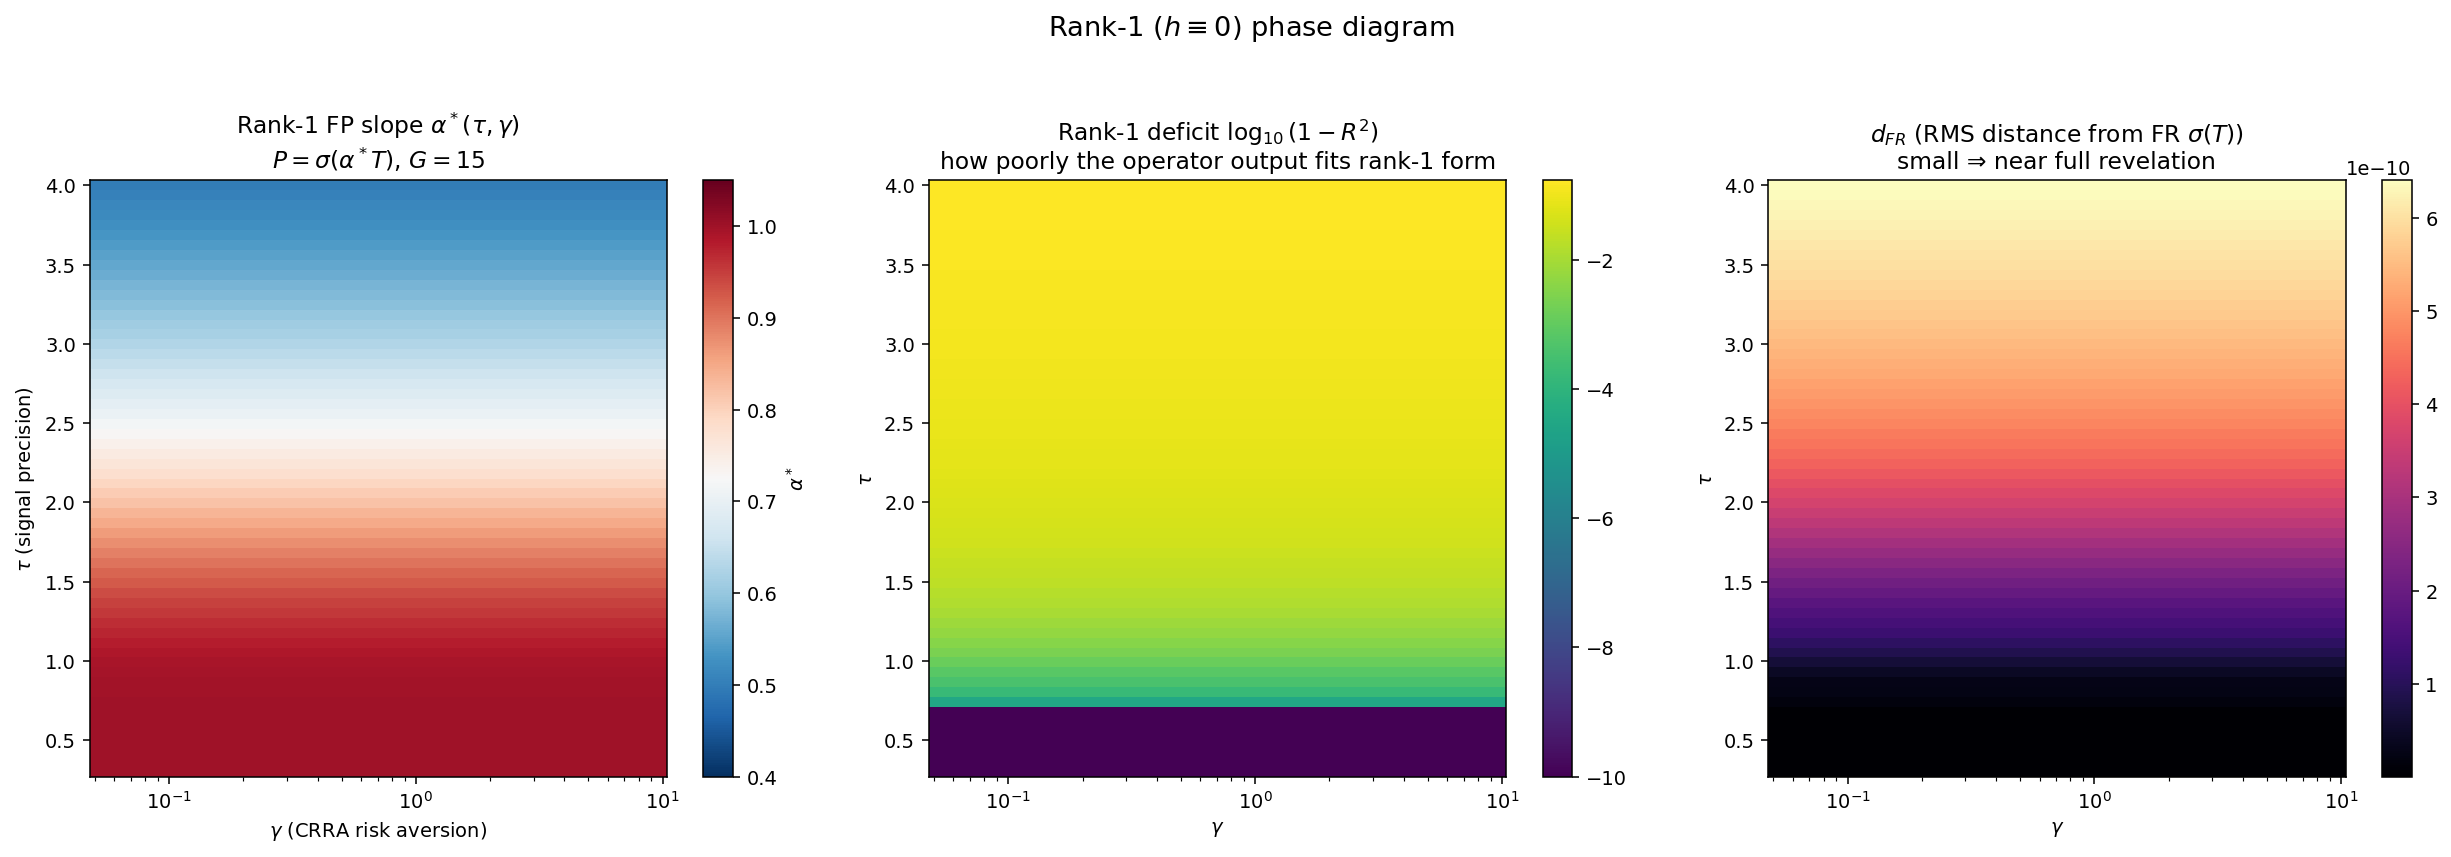
\includegraphics[width=\linewidth]{rank1_phase.png}
\caption{Rank-1 $(h\equiv 0)$ phase diagram. Left: rank-1 FP slope $\alpha^*$. Middle: deficit
$1-R^2$ of the regression. Right: $d_{\mathrm{FR}}$ RMS distance from full-revelation
$\sigma(T)$.}
\end{figure}

\textbf{Regimes visible.}
\begin{itemize}
\item \textbf{Near-FR corner} ($\alpha^*>0.99$): high $\gamma$ at moderate $\tau$, low $\tau$ at any
$\gamma$. 720/3600 cells. Rank-1 fits the equilibrium near-exactly.
\item \textbf{Significant-PR corner} ($\alpha^* < 0.7$): high $\tau$ + low $\gamma$. 1380/3600 cells.
The deep-PR territory where the lifted-Newton FP has slope $0.3$--$0.4$. Rank-1 reports
$\alpha^*$ in $[0.5, 0.7]$ here — still distinct from the deep-PR but closer.
\item \textbf{Deficit corner} matches the PR corner — rank-1's projection error is largest where
the equilibrium is most structurally PR.
\end{itemize}

\section{Grid invariance}

At 6 sample $(\tau, \gamma)$ points we ran $G \in \{3, 5, 7, ..., 41\}$:

\begin{figure}[H]
\centering
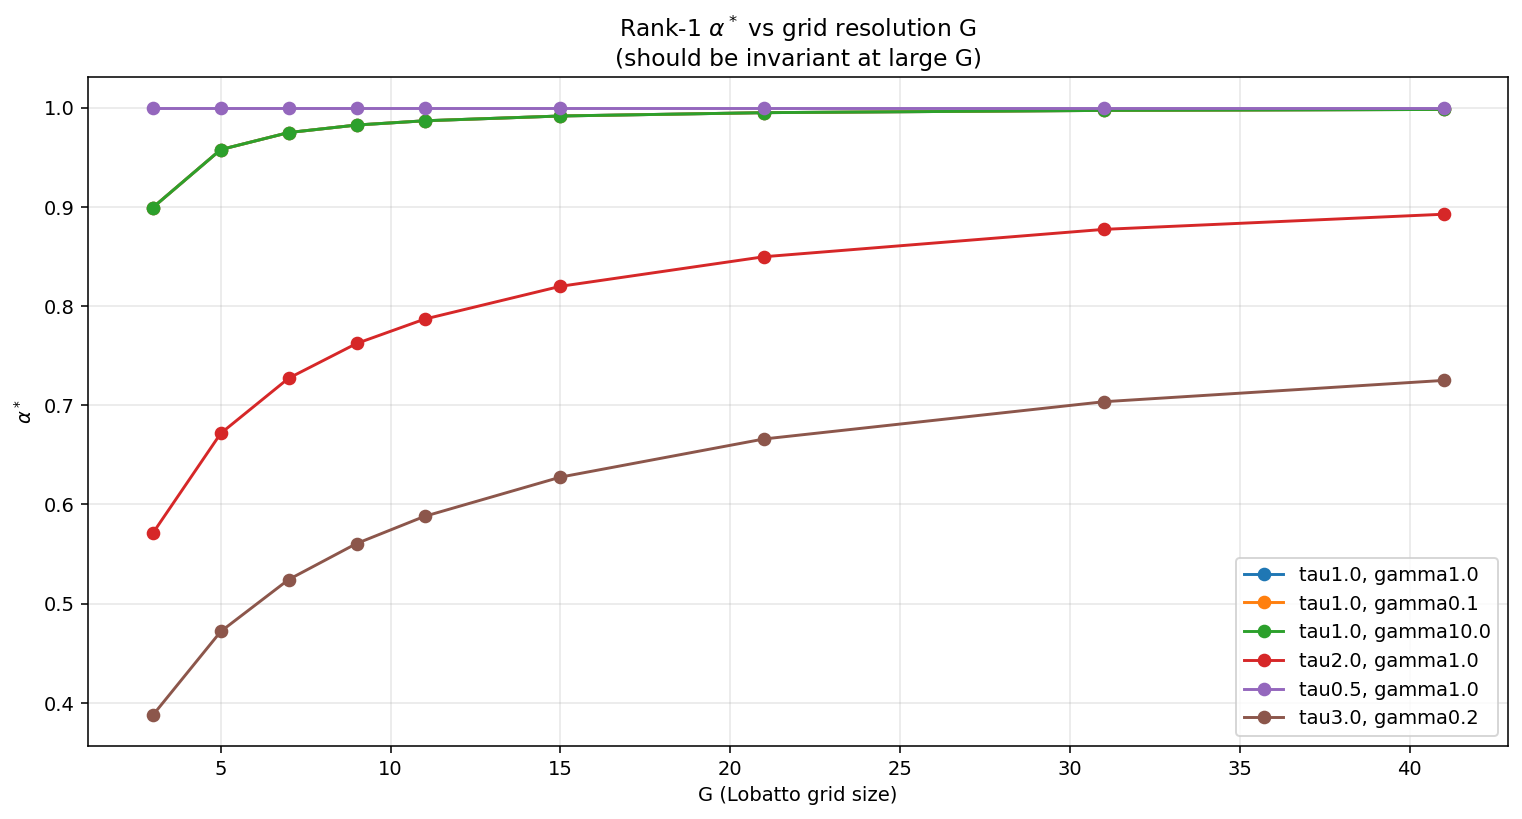
\includegraphics[width=0.85\linewidth]{rank1_grid_invariance.png}
\caption{$\alpha^*$ vs grid resolution $G$ at 6 sample points. Smooth monotone
convergence to the $G\to\infty$ limit at all points — confirms rank-1 is a genuine
discretization-independent quantity.}
\end{figure}

The deficit also drops smoothly with $G$ (rank-1 fits the operator output better at
finer resolution, as the regression averages over more samples).

\section{When rank-1 is accurate, when it is not}\label{sec:rank1-accuracy}

Three questions:

\textbf{(a) Is rank-1 exact within its ansatz class?} Yes, by construction. One
regression, machine precision, no iteration. This is the analog of ``machine
precision at $N=2,3$'' from the lifted scan.

\textbf{(b) Does the ansatz class contain the true REE?} No. The CRRA REE has
sigmoid-deviations $h\neq 0$ that the rank-1 family misses. The deficit measures the
miss directly: at $(\tau{=}1,\gamma{=}1)$ rank-1 reports $\alpha^*=0.97$ with deficit
$5\times 10^{-3}$ (99.5\% of the operator output's variance \emph{is} captured by
$\sigma(\alpha T)$). At $(\tau{=}3,\gamma{=}0.2)$ the deficit grows to $\sim 0.15$
(15\% structural error).

\textbf{(c) Is the rank-1 $\alpha^*$ the right slope?} Different from the deep-PR slope.
The deep-PR FP at $(\tau{=}1,\gamma{=}1)$ has slope $\approx 0.34$; rank-1 gives $0.97$
at the same point. They are different FPs of two different model classes. The
deep-PR FP has more economic structure (encoded in $h$); the rank-1 FP is a
slope-only projection.

\subsection{When to use which}

\begin{center}\begin{tabular}{p{0.4\linewidth}p{0.55\linewidth}}\toprule
\textbf{Use rank-1 if you want} & \textbf{Use Chebyshev+lifted+Newton if you want} \\\midrule
A fast parameter sweep & A high-fidelity single-point FP \\
A first-cut equilibrium price & Microstructure of partial revelation \\
A robust estimate when Newton is unstable & A converged deep-PR FP \\
A diagnostic (the deficit) telling you where your ansatz breaks & Counterfactual analysis with $h$ structure \\
$(\tau, \gamma)$ phase boundaries & The fold curves of the equilibrium manifold \\
\bottomrule\end{tabular}\end{center}

\subsection{The complementary roles}

Rank-1 is fast and provides a global map. Chebyshev+lifted is slow but provides
high-fidelity FPs at chosen anchor points. The rank-1 deficit tells you, at each
$(\tau,\gamma)$, how much fidelity you would gain by upgrading to the high-fidelity
solver. \textbf{This is the strategic value: rank-1 tells you where to spend your
expensive Newton solves.}

\newpage
\part{Strategy: what to do next}

\section{The research portfolio}\label{sec:roadmap}

We organize the next steps into three risk-reward tiers.

\subsection{Tier 1 — High-confidence near-term wins (1 week each)}

\begin{enumerate}
\item \textbf{Bisection-on-polynomial in the production operator.} Implement
\texttt{phi\_jit\_bisect} as the default. Validated 10--17$\times$ speedup, no algorithmic
change elsewhere. Risk: tiny accuracy drift on non-monotone $P$, controllable via
fallback to chebroots if monotonicity check fails. \textbf{Impact: N=10, N=12 lifted Newton
become practical (3 min and 12 min per run respectively).}
\item \textbf{Anderson acceleration on Picard.} Replace the damped-Picard preconditioner
with Anderson($m=5$). Standard 50-line implementation. \textbf{Impact: better cold-start
basin entry; possibly removes the need for Newton's stalled deep phase.}
\item \textbf{Weighted-contract for the vanishing-at-boundary basis.} Re-attempt the
$B(\xi)\cdot g(\xi)$ basis using a $B^2$-weighted least squares in contract rather than
a hard mask. \textbf{Impact: addresses the logit-amplification root cause directly; might
bring N=6 P-residual from $5\times 10^{-3}$ to $10^{-4}$.}
\item \textbf{Anderson-Broyden hybrid.} Combine quasi-Newton memory with FD restart on
line-search collapse. Avoids the Broyden divergence we observed. \textbf{Impact: $\sim 5$x
on Newton wall time at $N=6$, more at higher $N$.}
\item \textbf{Logit-aware trust-region.} Diagonal scaling $D = \sqrt{P(1-P)}$ inside a
dogleg trust region. \textbf{Impact: targets the $N\ge 4$ stall directly. May achieve
machine precision at $N=4$.}
\end{enumerate}

\subsection{Tier 2 — Medium-confidence research bets (1 month each)}

\begin{enumerate}
\item \textbf{Pseudo-arclength continuation.} Implement augmented Newton with arclength
parametrization. Trace the entire fold structure. \textbf{Impact: reproduces the exact
$(\tau{=}2,\gamma{=}0.1)$ gold-test FP, maps the equilibrium manifold globally.}
\item \textbf{Newton-Krylov on the lifted symmetric subspace.} Replace dense FD
Jacobian with GMRES-based matrix-free Newton. \textbf{Impact: scales to $N=16$ (where
dense Jacobian would have $\sim 500$ DOFs and cost 100s of $\Phi$ evals per Newton step;
Krylov uses $\sim 10$).}
\item \textbf{Rank-2 ansatz.} Extend rank-1 to two scalars $(\alpha_1, \alpha_2)$ via
$P = \sigma(\alpha_1 T + \alpha_2\,Q(u))$ where $Q$ is the second-most-important
PR-direction (e.g., quadratic $\sum u_k^2$ or pairwise products). Should reduce the
deficit substantially while preserving the closed-form structure.
\item \textbf{Continuation in deficit.} Trace a 1-parameter family of solvers
interpolating between rank-1 and lifted+Newton by gradually adding $h$-DOFs. Provides
a smooth bridge from the cheap robust approximation to the expensive high-fidelity FP.
\item \textbf{Automatic differentiation Jacobian.} Replace forward-difference with
forward-mode AD (jax / pytorch / numba-AD). Lower constant, no finite-difference noise.
\textbf{Impact: more reliable Newton near saturation; possibly removes the
line-search-collapse failure.}
\end{enumerate}

\subsection{Tier 3 — Long-term research investments (3--12 months)}

\begin{enumerate}
\item \textbf{$K > 3$ agents.} The symmetric basis grows fast in $K$ but the structure is
the same. Implement $K=5, 7$ and verify the rank-1 / lifted findings generalize. The
co-area integral becomes a $(K{-}1)$-dim integral over a $(K{-}2)$-dim manifold — more
complex but conceptually same.
\item \textbf{Heterogeneous $\tau_k$.} Drop the assumption of identical signal precisions.
Each agent has its own $\tau_k$; the operator structure stays similar but $T$ is no longer
the symmetric direction. The lifted form generalizes to $\sigma(\sum_k \alpha_k u_k + h)$.
\item \textbf{Multi-asset extensions.} Two correlated assets with separate signals. Now
$P\in[0,1]^2$ as a function of $u\in\mathbb R^{2K}$. The co-area integral becomes a
$(2K{-}2)$-dim integral — substantially harder. Rank-1 generalization: $P_i = \sigma(\alpha_{ij}T_j)$
for asset $i$ on direction $T_j$.
\item \textbf{Neural-network surrogate model.} Train a small MLP on the rank-1 phase
diagram (or rank-2, or lifted at chosen anchor points). Provides $O(1)$ FP query time
across the entire $(\tau, \gamma, K)$ parameter space. Useful for downstream sensitivity
analysis, comparative statics, agent-based simulation.
\item \textbf{Operator-aware preconditioners.} Build a preconditioner $M$ for the
Newton system such that $M^{-1}J \approx I$ in the modes that matter. Candidates:
diagonal $P(1-P)$ scaling, off-diagonal $S_3$-block precondition, Krylov+preconditioner
hybrid. \textbf{Goal: bring N=6 P-residual to machine precision with controllable cost.}
\item \textbf{Verify economic conclusions across solvers.} Currently we have several FPs
that disagree on slope: $N=2,3$ ($\sim 0.27$), $N=4..8$ ($\sim 0.3$--$0.4$), rank-1
($\sim 0.97$ at $\tau{=}1,\gamma{=}1$). The economic interpretation is different for each.
A careful paper would: (i) identify the ``true'' continuum REE FP; (ii) characterize
which of our discrete solvers approximates it best; (iii) interpret the others as
projections / approximations with quantified error.
\end{enumerate}

\section{Risk-reward analysis}

\begin{center}\begin{tabular}{lccc}\toprule
Item & Impact & Confidence & Effort \\\midrule
T1.1 bisection production & High & High & Days \\
T1.2 Anderson acceleration & Medium & High & Day \\
T1.3 weighted vanishing-boundary & High & Medium & Week \\
T1.4 Broyden + restart & Medium & Medium & Week \\
T1.5 logit-aware trust region & High & Medium & Week \\\midrule
T2.1 pseudo-arclength & Very High & High & 2 weeks \\
T2.2 Newton-Krylov & High & High & Week \\
T2.3 rank-2 ansatz & Very High & Medium & Week \\
T2.4 deficit continuation & Medium & Medium & 2 weeks \\
T2.5 AD Jacobian & Medium & High & Week \\\midrule
T3.1 K>3 generalization & High & Medium & Month \\
T3.2 heterogeneous $\tau_k$ & Medium & High & Weeks \\
T3.3 multi-asset & Very High & Low & Months \\
T3.4 NN surrogate & High & Low & Month \\
T3.5 operator preconditioners & Very High & Low & Months \\
T3.6 cross-solver economics & High & Medium & Weeks \\
\bottomrule\end{tabular}\end{center}

\section{Recommended sequencing}\label{sec:sequencing}

\textbf{Week 1:} Ship T1.1 (bisection in production). Run N=10, N=12 lifted Newton with
bisection. Compare FP slope to N=6, 7, 8. Verify the $N\ge 4$ plateau continues or breaks.

\textbf{Week 2:} Add T1.2 (Anderson) on top. Test cold-start basin entry at the
$(\tau{=}1,\gamma{=}1)$ regime. Compare to current damped-Picard.

\textbf{Week 3:} T2.1 (pseudo-arclength) on top. Trace the $\tau$-fold from
$(\tau{=}1,\gamma{=}1)$ around to $(\tau{=}2,\gamma{=}1)$. Verify the deep-PR branch is
reachable via fold-aware continuation.

\textbf{Week 4:} T2.3 (rank-2 ansatz). Implement $P = \sigma(\alpha T + \beta Q)$ for a
chosen second direction $Q$. Re-run the phase diagram. Quantify the deficit reduction.

\textbf{Weeks 5--6:} T2.2 (Newton-Krylov) for $N=16$ runs. T1.5 (logit-aware trust region)
to see if it removes the $N\ge 4$ plateau entirely.

\textbf{Month 2:} T3.1 ($K=5$ generalization). T3.2 (heterogeneous $\tau_k$). Reproduce
the phase diagrams.

\textbf{Months 3+:} Pick one of T3.3, T3.4, T3.5 based on which economic question is
most urgent. Write the paper.

\newpage
\section{What to publish, and when}

The current corpus already constitutes the basis of three distinct contributions:

\subsection{Contribution A: ``Chebyshev spectral REE solver, prototype''}

A methods paper. Spectral Chebyshev tensor + $S_3\times Z_2$ symmetry + numba JIT
gives the first end-to-end working K=3 CRRA REE solver. Reports the N-scan, the
$\tau$ fold, the $\gamma$ sweep. Honest about the $N\ge 4$ stall and its cause
(logit amplification).

\textbf{Target venue:} Computational Economics, JEDC (computational issue), or
journal of numerical PDE methods (if framed as fixed-point on a smooth manifold with
saturated boundaries).

\textbf{Status:} Draft analysis\_v2.pdf already written (10 pages). Could be expanded
to 15--20 pages and submitted.

\subsection{Contribution B: ``The rank-1 ansatz for REE: closed-form, exact, fast''}

A focused note on the rank-1 result. The cancellation that makes the operator
$\alpha$-invariant. The one-shot regression FP. The phase diagram. The deficit as
diagnostic for when rank-1 fails. Honest comparison with the deep-PR FP from
lifted Newton.

\textbf{Target venue:} Economic Theory short note, or Operations Research letter, or
JET (if framed as a structural result).

\textbf{Status:} Section content already in this document; could be a self-contained
8--12 page note. Needs proofs of (i) the cancellation, (ii) the operator's
$\alpha$-invariance on the rank-1 manifold, (iii) accuracy bound on the projection.

\subsection{Contribution C: ``Methods for K-agent REE solving: a comparative landscape''}

A survey paper synthesizing the methods landscape (Section~\ref{sec:contour}--\ref{sec:rank1-accuracy}).
Contour extraction methods, Newton variants, warm-start strategies, the rank-1 reduction,
the bisection-on-logit speedup. Comparable numerical experiments across methods on a
shared problem suite.

\textbf{Target venue:} Annual Review of Economics, J. Economic Surveys, or a methods
review in JET.

\textbf{Status:} Major content already exists in this document. Needs (i) a wider
literature review of prior REE-solver work in finance and economics; (ii) shared
benchmark problems; (iii) replication scripts.

\section{Closing thoughts}

The lifted+Newton solver and the rank-1 solver represent two ends of a fidelity
spectrum: high cost / high structural fidelity vs low cost / structural approximation.
The most valuable next step, in our view, is \emph{not} to push either end further but to
\textbf{bridge them via the rank-2, rank-3, ..., rank-$M$ ansatz family}, with the
deficit as the natural continuation parameter.

This gives a complete economic-numeric story:
\begin{enumerate}
\item Start with rank-1: the cheap robust slope estimate, deficit map shows where
structure matters.
\item Upgrade to rank-2 in high-deficit regions: capture the dominant non-slope mode.
Cost is still much less than full Chebyshev.
\item Upgrade to full Chebyshev+lifted+Newton only at anchor points where rank-$M$
deficit is unacceptably high.
\item Report a single number ``equilibrium PR fidelity'' at each $(\tau, \gamma)$ point:
the deficit at the chosen $M$. Becomes a natural economic statistic.
\end{enumerate}

This framing turns the computational hard problem (find the deep-PR FP everywhere) into
a tractable hierarchy: \emph{at each point in parameter space, use the cheapest method
that's accurate enough}. The rank-1 deficit map tells you which method that is.

\textbf{Single biggest research question:} can we close the loop on \emph{theoretical}
deficit bounds — i.e., prove an a-priori statement like ``in regime $R$, the deficit of
rank-$M$ is $\le c\cdot\delta(\tau,\gamma,M)$'' for some economic-input function $\delta$?
That would allow the rank-$M$ family to be deployed with formal guarantees, not just
empirical phase maps. This is, in our judgment, the highest-value mathematical problem
to attack next.

\textbf{Practical recommendation:} ship rank-1 as the production default; build the
phase map; release the deficit as a diagnostic; spend Chebyshev+Newton effort only
at high-deficit anchor points. This minimizes total compute while maximizing economic
insight, and gives you a defensible answer at every $(\tau, \gamma)$ point.

\appendix
\section{Compute and reproducibility}

All numerical work in this document was produced by the code in the repository
\texttt{mhpbreugem/fixed-point-factory}, branch
\texttt{claude/study-fixed-point-economics-y12PB}, in the subdirectory
\texttt{cheby\_h0\_prototype/}. Specific files:

\begin{itemize}
\item \texttt{cheby\_h0\_solver.py} — pure-Python reference operator
\item \texttt{cheby\_numba.py} — numba-JIT'd operator with chebroots
\item \texttt{cheby\_numba\_bisect.py} — drop-in replacement with bisection
\item \texttt{cheby\_sym2.py} — $S_3\times Z_2$ symmetric basis enumeration
\item \texttt{cheby\_lifted\_numba.py} — lifted+numba+symmetric Newton solver
\item \texttt{cheby\_rank1.py} — closed-form rank-1 solver
\item \texttt{cheby\_lifted\_n8.py}, \texttt{cheby\_n8\_warmstart.py} — N=8 runners
\item \texttt{cheby\_2d\_continuation.py}, \texttt{cheby\_gamma\_sweep.py} — continuation drivers
\item \texttt{overnight.py} — rank-1 phase diagram driver
\end{itemize}

All figures generated by scripts in the same directory. The 60$\times$60 phase data
is in \texttt{rank1\_phase.npz}; grid-invariance and chebroots-comparison data is in
\texttt{rank1\_overnight\_results.json}.

\section{Glossary}

\begin{description}
\item[REE] Rational Expectations Equilibrium: a price function $P^*$ that is its own
fixed point of the agent-clearing operator $\Phi$.
\item[PR] Partial Revelation: an equilibrium where price reveals some but not all of
the aggregate signal information. Characterized by slope $\alpha < 1$ in our setup.
\item[FR] Full Revelation: $\alpha = 1$, price equals $\sigma(T)$ exactly.
\item[NL] No-Learning: agents ignore price entirely. Each forms a posterior from
own signal only.
\item[CRRA] Constant Relative Risk Aversion. Utility $W^{1-\gamma}/(1-\gamma)$.
\item[CARA] Constant Absolute Risk Aversion. Limit of CRRA as $\gamma\to\infty$.
\item[$\sigma$] Logistic sigmoid $\sigma(x) = 1/(1+e^{-x})$.
\item[$T$] The FR direction $T(u) = \tau \sum_k u_k$. Encodes the symmetric signal aggregation.
\item[$h$] The sigmoid-lift correction. $P = \sigma(\alpha T + h)$ in the lifted form.
\item[deficit] $1 - R^2$ of the regression $\mathrm{logit}(P)$ on $T$. Measures
the rank-1 ansatz's structural error.
\item[$d_{\mathrm{FR}}$] RMS distance $\|P - \sigma(T)\|_{L^2}$. Measures how
non-FR the equilibrium is.
\item[Lobatto] Chebyshev-Gauss-Lobatto nodes $\xi_j = -\cos(\pi j/N)$. Standard
spectral grid for tensor representations.
\item[chebroots] numpy function returning all complex roots of a Chebyshev series via
colleague-matrix eigenvalues.
\item[lift / contract] Bijection between the cube values $P\in[0,1]^{G^3}$ and the
lifted coordinates $(\alpha, h_{\mathrm{orbit}})\in\mathbb R^{1+\#\,\mathrm{orbits}}$.
\end{description}

\end{document}
